% !TeX spellcheck = en_EN-English

\chapter{Theory - models}
\label{chap:thoery}

During our research, we utilized several different machine learning models. In this chapter, we introduce these models from a more theoretical point of view.

\section{Multilayer perceptron}
\label{MLP}

A multilayer perceptron is a feed-forward neural network, meaning that data flows in a single direction and neurons do not form cycles. This network consists of fully connected, sometimes called dense, layers with non-linear activation functions, as shown in Fig. \ref{fig:mlp}. We can see that this model can be split into three parts: the input layer, which loads the data; the hidden layers, which extract the desired information using linear transformations and activation functions; and finally, the output layer, which applies a final linear transformation followed by an activation function to produce the output. Each layer can be described using the formula shown in Eq. \ref{eqn:mlp}, where $h_i$ is the resulting vector of the $i$-th layer, $act()$ is a non-linear activation function, $W_i$ is the weight matrix of the $i$-th layer, $h_{i-1}$ is the resulting vector from the previous layer, and $b_i$ is the bias vector.

\begin{equation}
	\label{eqn:mlp}
	h_i = act(W_i h_{i-1} + b_i),
\end{equation}

\begin{figure}[!h]
	\centering
	
	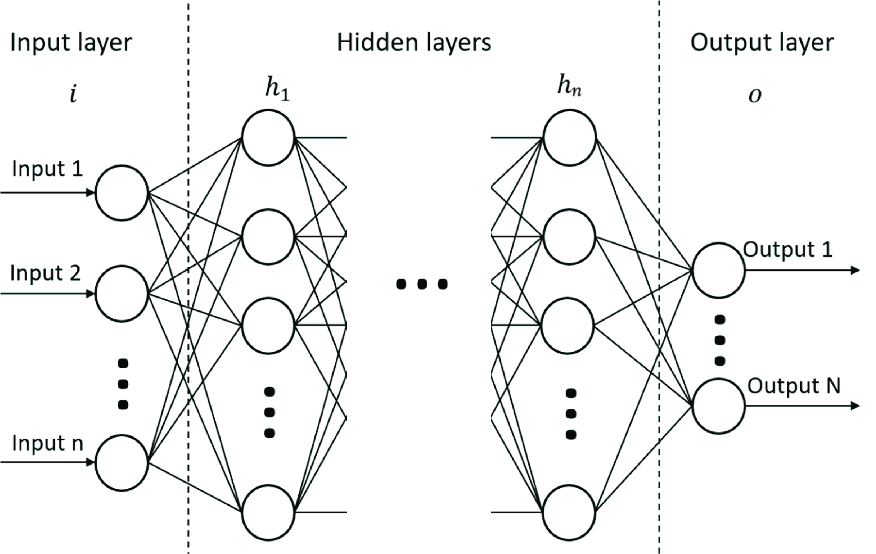
\includegraphics[width=0.8\textwidth]{images/MLP_arch.png}
	
	\caption{Architecture of multilayer perceptron \cite{MLParch}.}
	\label{fig:mlp}
\end{figure} 

\section{Recurrent neural network}
\label{theoryRNN}

In general, a recurrent neural network is a type of neural network that, in some way, uses results from previous steps to improve its predictions. These models are used for ordered data, where each subsequent step depends on more than just the immediately preceding one.

\subsection{Elman RNN}

The Elman RNN, also known as a simple recurrent network (SRN), is a type of recurrent neural network that utilizes the results of the hidden layer before activation in the previous step as an additional input in the next one. We can see this architecture in Fig. \ref{fig:elman_arch}, where on the left we observe how forward propagation occurs and on the right how it is unrolled over time. Here, the middle layer, which is the hidden layer of the model, receives two inputs: the input vector $x_t$, where $t$ denotes the step (usually a time step), which is multiplied by a matrix of weights $W_i$, and the vector $h_{t-1}$, which is the result of this layer (also called the context vector) from the previous step, multiplied by a different matrix of weights denoted as $W$. These two results are summed together, and the result is passed to the activation layer, which generates the new vector $h_t$ \cite{elman}. This entire process is summarized in Eq. \ref{eqn:elman}, where $b_i$ and $b$ are bias vectors.

\begin{equation}
	\label{eqn:elman}
	h_t = act(x_t W^T_i + b_i + h_{t-1} W^T + b).
\end{equation} 

Usually, this result is directly used as the output or passed through a single fully-connected feed-forward layer. In a multi-layered version of this network, the output of the first hidden layer is fed into the next hidden layer, along with the output of that specific layer from the previous step. Both inputs are multiplied by weight matrices specific to that layer, summed together, and then passed through an activation function.

\begin{figure}[!h]
	\centering
	
	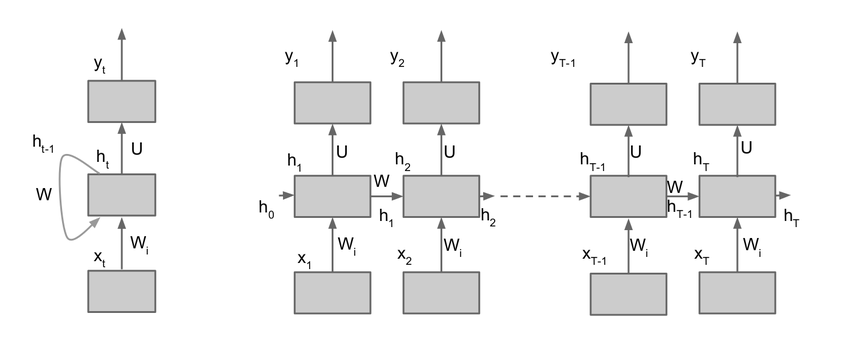
\includegraphics[width=0.85\textwidth]{images/Elman_RNN_architecture.png}
	
	\caption{Architecture of Elman RNN \cite{elman_img}.}
	\label{fig:elman_arch}
\end{figure}

\subsection{Gated Recurrent Unit}

A Gated Recurrent Unit (GRU) is a more complex RNN variant compared to the Elman RNN. Developed as a simplification of the even more intricate LSTM model, the GRU primarily consists of three interacting components: the reset gate, update gate, and candidate hidden state computation. These components collaboratively regulate information flow to produce the final prediction.
\\

The structure of a GRU’s hidden layer is illustrated in Fig. \ref{fig:gru_arch}. In this diagram:

\begin{itemize}
	\item Sigmoid: Represents a fully connected feed-forward layer with a sigmoid activation function.
	\item Tanh: Represents a fully connected feed-forward layer with a hyperbolic tangent activation function.
\end{itemize}

The reset gate, located on the left side of the diagram, uses the input and previous hidden state vectors to modify the previous hidden state vector, which is then fed into the candidate hidden state computation. This process helps capture short-term dependencies in time series by selectively removing information from the previous hidden state vector.
\\

The candidate hidden state computation is similar to the Elman RNN but with two key differences: first, the inputted hidden layer is modified by the reset gate's result; second, the resulting vector from this part serves only as a candidate that undergoes further calculation. This candidate vector primarily contains current and short-term past information due to the specific vectors that form its input.
\\

The update gate, similar to the reset gate, uses the concatenation of the input and previous hidden state vector as its input. However, its results are used to modify both the previous hidden state and the candidate hidden state, creating a final hidden state that is a weighted average of these two vectors, with weights derived from this gate. This architecture helps capture long-term dependencies in time series by reintroducing relevant information from the previous hidden state vector into the final hidden state, combining it with the candidate hidden state vector that contains mostly current and short-term information. The entire architecture is depicted in Fig. \ref{fig:gru_arch}.
\\

\begin{figure}[!h]
	\centering
	
	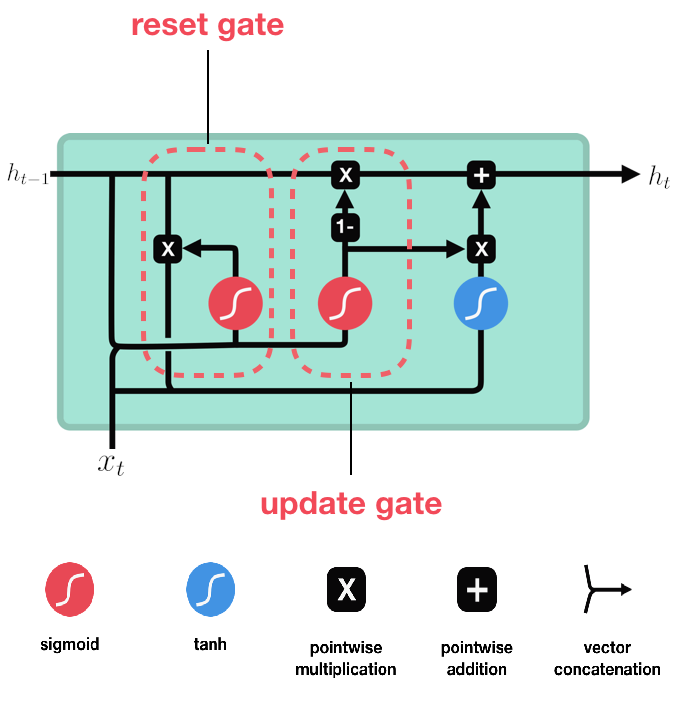
\includegraphics[width=0.6\textwidth]{images/GRU_arch.png}
	
	\caption{Architecture of GRU hidden layer.}
	\label{fig:gru_arch}
\end{figure}

The multi-layered version of this architecture is achieved by stacking hidden layers, where the hidden state vector of one layer becomes the input vector for the next.

\subsection{Long Short-Term Memory}

As mentioned earlier, the LSTM is a more complex predecessor of the GRU. Developed to address the vanishing gradient problem that limits long-term memory in models like the Elman RNN, the LSTM introduces a memory vector, often called a memory cell, designed to maintain information over longer periods. As shown in Fig. \ref{fig:lstm_arch}, this model consists of three gates and a candidate memory computation. The legend in this diagram has the same meaning as in the GRU architecture diagram.
\\

All three gates and the candidate memory computation share the same input, which consists of the input vector and the previous hidden state vector. In each case, this input passes through a fully connected feed-forward layer and then into an activation function. For the gates, this activation function is the sigmoid function, which bounds all values within the range (0,1), while the candidate memory calculation uses the hyperbolic tangent as its activation function.
\\

The forget gate is responsible for removing unnecessary information from the memory vector by performing an element-wise multiplication of its result with the previous memory vector.
\\

The input gate, together with the candidate memory vector computation, is designed to introduce new information into the memory cell after adjustments made by the forget gate. First, the model computes the candidate memory vector; this vector is then adjusted by the input gate's result and added to the modified previous memory vector, resulting in a new memory vector.
\\

Finally, the output gate determines how much each part of the memory should contribute to the new hidden state vector. This process is illustrated in Fig. \ref{fig:lstm_arch}.

\begin{figure}[!h]
	\centering
	
	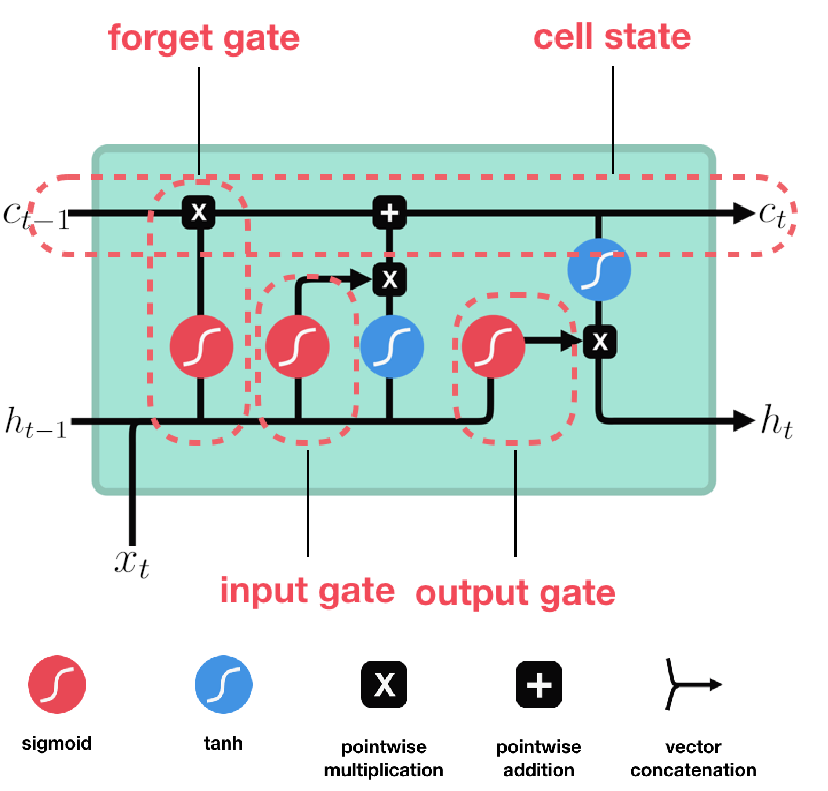
\includegraphics[width=0.6\textwidth]{images/LSTM_arch.png}
	
	\caption{Architecture of LSTM hidden layer.}
	\label{fig:lstm_arch}
\end{figure}
\newpage

\section{Transformer}
\label{theoryTrans}

The Transformer is a deep learning model architecture introduced in 2017 by Vaswani et al. \cite{attentionAllYouNeed} that is especially good at handling sequences, such as text. This architecture consists of an encoder and a decoder, as shown in Fig. \ref{fig:trans}. The encoder in this model is meant to create a contextualized representation of the input, while the decoder takes this contextualized representation and combines it with previous outputs to predict the next output. In addition to these two main blocks, this model usually also contains a tokenizer, an embedding layer, and positional encoding to prepare the input data, as well as a fully connected feed-forward layer with a softmax activation function to turn the result of the decoder into a probability distribution over possible tokens.

\begin{figure}[!h]
	\centering
	
	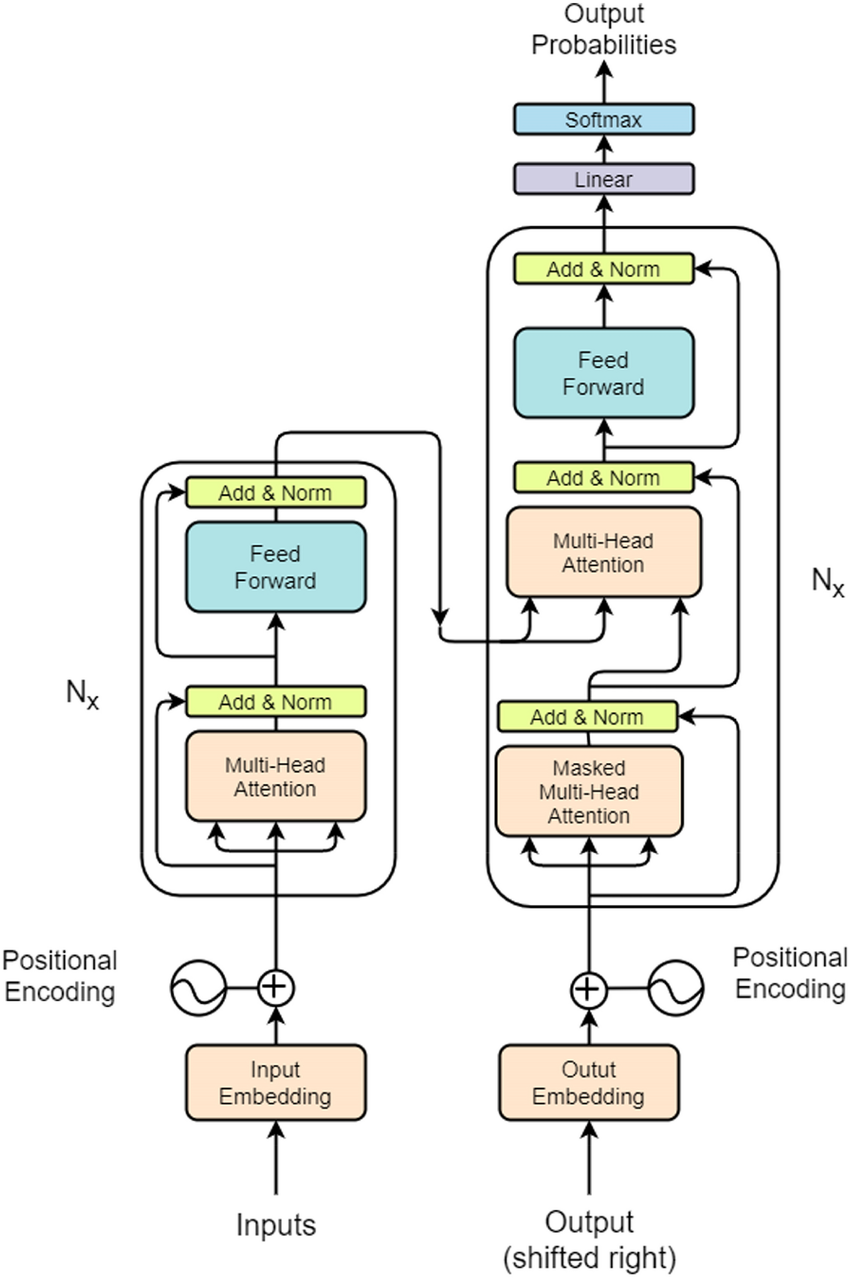
\includegraphics[width=0.6\textwidth]{images/trans_arch.png}
	
	\caption{Architecture of one encoder-decoder block in transformer model from original "Attention is all you need" paper \cite{attentionAllYouNeed}.}
	\label{fig:trans}
\end{figure}

\subsection{Tokenizer, Embedding layer and Positional encoding}

The first part of the Transformer model is usually input preparation, which may vary depending on the type of data used. This part consists of three components:

\begin{itemize}
	\item Tokenizer: This layer splits the input into tokens. For example, if the input is textual, tokens might be words or syllables.
	\item Embedding layer: The task of this layer is to transform each input token into a numerical vector of the same length.
	\item Positional encoding: The final preparation layer adds a vector to each token’s embedding, encoding its position relative to other tokens.
\end{itemize}

In most cases, the Tokenizer and Embedding layer are trained separately and do not change during training of the Transformer, while the Positional Encoding is trained alongside the rest of the Transformer.

\subsection{Encoder}
\label{theoryEncoder}

Encoder architecture consists of multiple attention blocks, where each block consists of multi-headed self-attention and a multi-layered feed-forward neural network. After each of these steps, the embeddings from the step input are added to the output, and the result is layer-normalized. Adding the step input embedding creates residual paths that help mainly with the vanishing gradient problem, while layer normalization ensures that the results neither explode nor vanish, and also brings a bit of additional non-linearity to the model. First, input embeddings are split into parts, each of which goes into a separate self-attention head.
\\

The architecture of self-attention is shown in Fig.~\ref{fig:self_att}, where we can see that each input token is multiplied by key, query, and value matrices to obtain their key, query, and value vectors. After that, each query is multiplied with each key to create the attention matrix, which encodes how much each token influences the others. This matrix then goes into a column-wise softmax function to normalize it, and finally, it is multiplied by the matrix of value vectors to create new embeddings of the tokens that should contain not only the original information but also the influence information.
\\

\begin{figure}[!h]
	\centering
	
	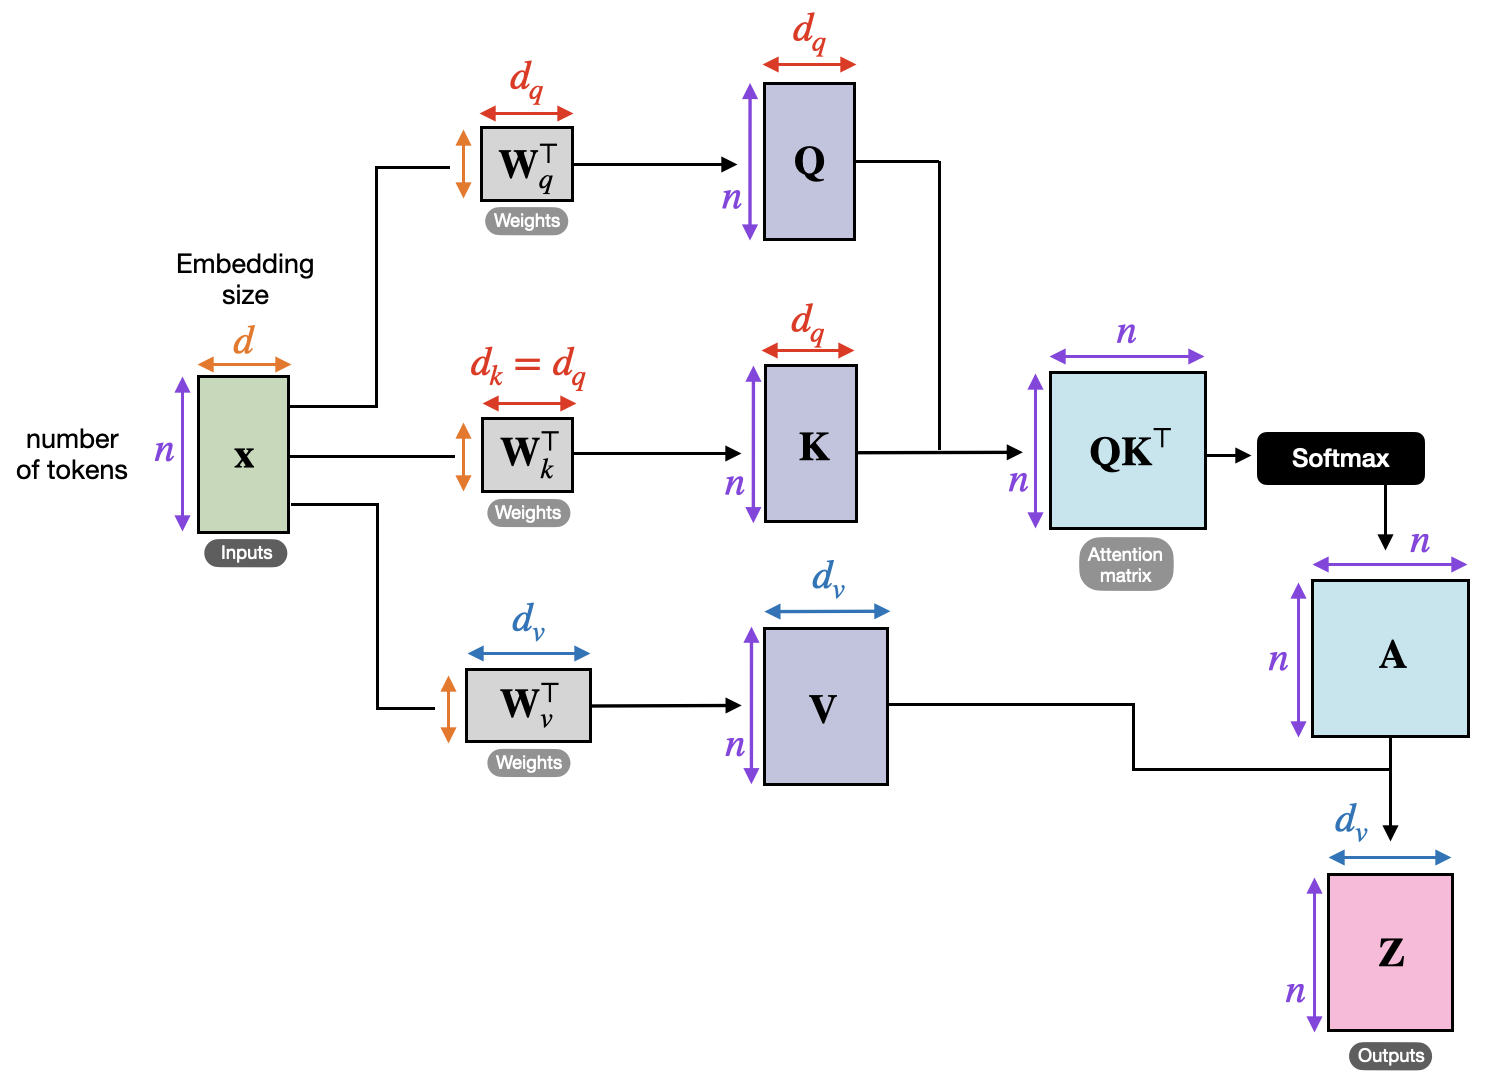
\includegraphics[width=1\textwidth]{images/self_attention.png}
	
	\caption{Architecture of Self-attention mechanism.}
	\label{fig:self_att}
\end{figure}

The results of each self-attention head are then concatenated back into new embeddings that have the same dimensions as the original ones. After adding the residual connection and normalization, the results go into a multi-layered feed-forward neural network to further extract information from the embeddings.

\subsection{Decoder}

The architecture of the decoder, similarly to the encoder, consists of multiple attention blocks; however, in this case, each attention block consists of three parts instead of two.
\\

The first part is masked multi-headed self-attention, which is similar to unmasked self-attention, with the only difference being the application of masking to the attention matrix before the softmax function. This ensures that words at certain positions do not affect words at other specific positions. The decoder uses what is called causal or look-ahead masking, which prevents future tokens from affecting past ones. In our case, this guarantees that a record cannot be influenced by records that occur later, that is, in the future from its perspective.
\\

The second part is multi-headed cross-attention, which takes two lists of token embeddings and computes the effect of tokens in the first list on tokens in the second list. In this case, the key and value vectors are computed from the contextualized representation produced by the encoder, while the query vectors are computed from the results of self-attention in the decoder. Other than this, the remaining architecture is the same as unmasked self-attention.. 
\\

The final part of the decoder attention block is a multi-layered feed-forward neural network that further extracts information from the embeddings.

\subsection{Fully-connected Feed-forward layer}

After that, the results of the decoder pass into the final fully-connected feed-forward layer, which changes the dimensionality of the decoder output from the embedding size to the vocabulary size and applies a softmax activation to the result. This setup is designed to produce a probability distribution over all possible tokens for the last token.
\\

In our case, we modified this final step. We encountered a problem where most records (our tokens) were unique, creating an extremely large vocabulary. This issue arose partially due to the many possible combinations of diseases, drugs, and medical procedures encoded in each record, and partially due to timestamps adding uniqueness, as it is unlikely for two patients to receive the same drug for the same disease at the same age.
\\

To address this, we removed the softmax activation and altered the fully-connected feed-forward layer so that the result maintains the embedding dimension. We then added a function that splits the result, finds the closest embedding for each part, and concatenates these embeddings together, yielding a specific new embedding prediction instead of a probability distribution.

\subsection{Decoder-only Transformer}

The Decoder-only version of the Transformer model is a simplified variant that entirely excludes the Encoder part and removes the Cross-Attention mechanism from the Decoder. This model is typically used when generating subsequent tokens without relying on a stable contextual input that would normally be processed by the Encoder.
\\

This simplification makes the architecture more akin to a standard RNN in terms of input-output behavior, where the model generates sequences step-by-step without explicit cross-contextual dependencies.

\section{Language-agnostic BERT Sentence Embedding}
\label{theoryLaBSE}

The Language-agnostic BERT Sentence Embedding model, also known as LaBSE, is a model trained with the main goal of generating similar representations for pairs of sentences that have the same meaning and are only translations of each other in two different languages \cite{labse_kaggle}.
\\

The architecture of the LaBSE model consists of four parts \cite{labse_hug}:

\begin{enumerate}
	\item Encoder-only transformer (BERT model)
	\item Pooling layer
	\item Dense layer
	\item Normalization layer
\end{enumerate}

\subsection{Encoder-only Transformer (BERT model)}
\label{emb:trans}

The first and most important part of the LaBSE model is the transformer, a deep learning architecture. More specifically, LaBSE uses BERT (Bidirectional Encoder Representations from Transformers), an encoder-only transformer architecture. This means the model lacks the decoder found in the standard Transformer (typically used for prediction tasks), allowing BERT to focus solely on extracting contextual information from input text.
\\

The architecture of the standard BERT model includes:

\begin{enumerate}
	\item Tokenizer layer
	\item Embedding layer
	\item Encoder
	\item Task layer
\end{enumerate}

\subsubsection{Tokenizer layer}

The first layer is the tokenizer, which takes the input text and splits it into tokens. In the case of the BERT model, this is called the PieceWise tokenizer, which splits text into subwords, something similar to syllables. The PieceWise tokenizer has advantages compared to other tokenizers that use either words or characters. Compared to character-wise tokenization, subwords contain more information than individual characters. Compared to word tokenization, there are far fewer subwords than words, and subwords are more similar across multiple languages, resulting in a much smaller vocabulary. This is especially important for multilingual models. After splitting, this layer assigns an integer number to each unique token. The LaBSE model’s vocabulary distinguishes around 500,000 different tokens.

\subsubsection{Embedding layer}

After that comes the embedding layer, which assigns a real-number vector to each token. Specifically, the BERT model computes three distinct embeddings, sums them, and normalizes the result to produce the final embedding:

\begin{itemize}
	\item Token type embedding: The base embedding where each token in the vocabulary is assigned a unique vector.
	\item Positional embedding: Encodes the token’s position within the sequence, providing contextual information about its location.
	\item Segment type embedding: Indicates which segment (typically a sentence) the token belongs to, crucial for processing multi-sentence input.
\end{itemize}

\subsubsection{Encoder}

The third and most important layer is the encoder. This is the layer in which contextual information is mined from the text. The architecture of this layer is the same as the encoder described in Sec. \ref{theoryEncoder}. In the BERT variant used by LaBSE, the encoder contains 12 attention blocks.

\subsubsection{Task layer}

The training process of the BERT model usually consists of two tasks on which the model is trained at the same time. The first is Masked Language Modeling (MLM), where 15\% of input tokens are masked, meaning they are either replaced by a mask placeholder or by a random different token. The masked input then goes into the model, and the resulting tokens at the positions of the masked tokens in the input are compared to the correct tokens before masking. This creates an error that is back-propagated through the model, updating its parameters \cite{bert_pretr_1}. The other task usually used is called Next Sentence Prediction (NSP). In this task, the model receives input that starts with a special classification token and then two spans of text separated by a special separator token. The task of the model is to determine whether these two spans of text can appear one after another, or more precisely, whether they appeared consecutively in the training corpus. This information is encoded in the first token of the result using two special tokens, either "is next" or "not next." Similarly, the difference between the expected and resulting first token creates an error that is back-propagated through the model \cite{bert_pretr_2}.
\\

However, in some BERT-based models like LaBSE, the second task is replaced with Translation Language Modeling (TLM). This task is an extension of MLM, in which the model receives two concatenated sentences instead of one, where the second sentence is a translation of the first in another language. The rest of the task is the same as in MLM: the whole input is masked, and the model is tasked with predicting the masked tokens \cite{bert_pretr_3}. 
\\

The task layer is used primarily only during pre-training and is omitted when the model is used for a different task, as many use cases do not need tokens in the results but instead use embeddings from the encoding layer as a form of text encoding, which is then used in task-specific layers for fine-tuning.


\subsection{Pooling layer}

After the BERT model returns embeddings for all input tokens, these embeddings need to be aggregated into a single vector that represents the embedding of the entire input. This aggregation is typically performed using a pooling layer. In the case of LaBSE, this pooling is done simply by taking the embedding of the first token, which is the embedding of the special classification token added to the beginning of the BERT input.

\subsection{Dense layer}

The next layer is a standard feed-forward dense layer using a hyperbolic tangent activation function. The number of input and output neurons is the same, and the layer includes an additional bias neuron.

\subsection{Normalization layer}

The final layer is normalization, whose task is to normalize the resulting vector by dividing it by its $L_2$ norm, ensuring the final vector has an $L_2$ norm equal to one.

\section{Word2vec model}
\label{theoryW2v}

Word2vec is a neural network-based method for generating word embeddings, which are dense vector representations of words that capture their semantic meaning and relationships. In other words, properties like the distance between two embeddings contain underlying information about those words, such as their similarity. There are two main approaches to implementing Word2vec:

\begin{itemize}
	\item Continuous bag-of-words (CBOW) 
	\item Skip-gram
\end{itemize}

\subsection{CBOW approach}

A model using the CBOW approach receives a sequence of words called the context, with one word missing, and tries to predict the missing target word as output. The model initially assigns one-hot encoding to each word in its dictionary. During training, each word from the context is first converted into its one-hot encoded embedding, which is then multiplied by a weight matrix to obtain its lower-dimensional dense embedding. The dense embeddings of all words in the context are then averaged, and the resulting embedding goes into a hidden layer, which transforms the vector back into the dimension of the vocabulary. Finally, a softmax function is applied to get the probability of each word in the vocabulary being predicted as the missing word. We can see this architecture in Fig. \ref{fig:cbow_arch}. Training is usually done using a fixed context window moving along the training text.

\begin{figure}[!h]
	\centering
	
	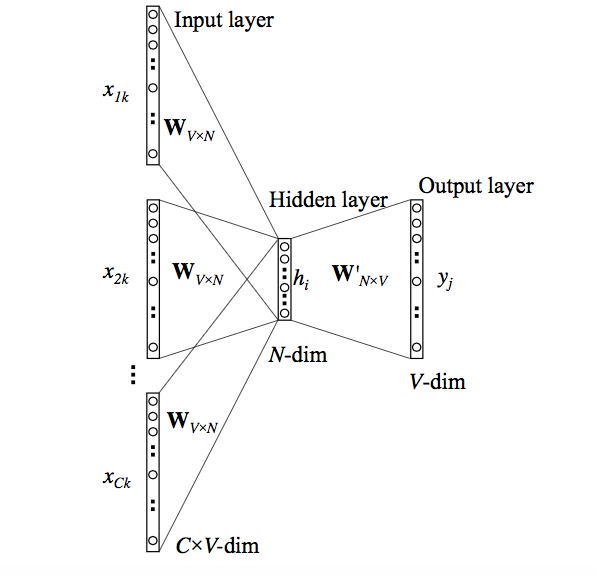
\includegraphics[width=0.9\textwidth]{images/CBOW_arch.png}
	
	\caption{Architecture of NN to train CBOW implementation of Word2vec model \cite{cbow}.}
	\label{fig:cbow_arch}
\end{figure}

\subsection{Skip-gram approach}

The Skip-gram approach works in the opposite way, the model receives a target word and tries to predict the surrounding context words. Similar to CBOW, the input word is first one-hot encoded and then multiplied by a weight matrix to transform it into a dense embedding. This embedding is passed to the next layer, which transforms it back into the vocabulary dimension. A softmax function is then applied to generate a probability distribution over potential context words.
\\

The Skip-gram’s loss function is the sum of the negative log-likelihoods of all context words. This architecture is illustrated in Fig. \ref{fig:skip_arch}.
\begin{figure}[!h]
	\centering
	
	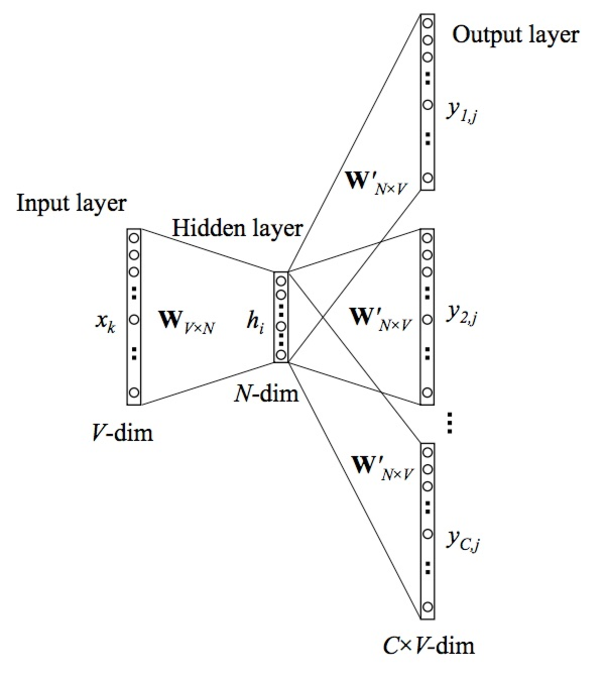
\includegraphics[width=0.9\textwidth]{images/Skip_arch.png}
	
	\caption{Architecture of NN to train Skip-gram implementation of Word2vec model \cite{skipgram}}
	\label{fig:skip_arch}
\end{figure}